\begin{frame}
	\frametitle{\problemtitle}
	\begin{block}{Problem}
		Given:
		\begin{itemize}
			\item the density $d_a$ of air and $d_w$ of water,
			\item the radius $r$ and height $h$ of a cylindrical container.
		\end{itemize}
		To which height should the cylinder be filled with water to minimise the
		height of the centre of mass?
	\end{block}
	\pause
	\centering
	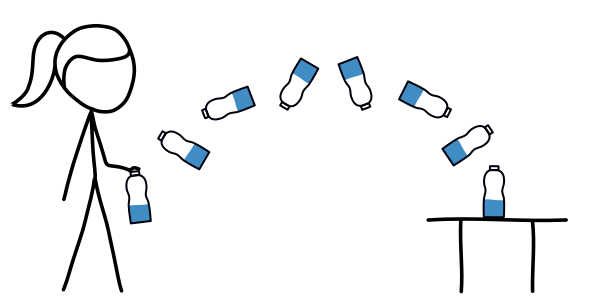
\includegraphics[height=0.5\textheight]{sketch}
\end{frame}

\begin{frame}
	\frametitle{\problemtitle}
	\begin{block}{Observations}
		\begin{itemize}
			\item The radius $r$ is irrelevant.
			\pause
			\item The result can be found using ternary search.
		\end{itemize}
	\end{block}
	\pause
	\begin{block}{Solution}
		\begin{itemize}
			\item Given the height $h_w$, calculate $h_a=h-h_w$.
			\item The centre of mass of the water is at height $c_w=\frac{h_w}{2}$.
			\item The centre of mass of the air is at height $c_a=h-\frac{h_a}{2}$.
			\pause
			\item The height of the combined centre of mass is the weighted average\pause:
			\[\frac{c_a\cdot{}d_a\cdot{}h_a+c_w\cdot{}d_w\cdot{}h_w}{h_a\cdot{}d_a+h_w\cdot{}d_w}.\]
			\item Can also be found by solving a quadratic equation.
		\end{itemize}
	\end{block}
	\pause % For some reason, this slide needs an extra \pause
	\solvestats
\end{frame}
